\documentclass[11pt]{beamer}

\usetheme[sectionpages,logo={_figures/poli-blue.pdf}]{UniNA}
\usefonttheme[onlymath]{serif}

\usepackage{tikz}
\usepackage{graphicx}
\usepackage{caption}
\usepackage{subcaption}
\usepackage{stanli}
\usepackage{siunitx}
\usepackage{mathtools}
\usepackage{quotes}
\usepackage{amsmath}
\usepackage{empheq}

\title{Sistema de suspensão rocker-bogie} %shown in title frame
\subtitle{PEF-3208 - Fundamentos em Mecânica das Estruturas}  % could also be a conference name

\date{\today} %explicitly set date instead of \today

\author[Natanael M. Cardoso]{Natanael Magalhães Cardoso}

\institute{Escola Politécnica - Universidade de São Paulo}

\begin{document}

\maketitle

\section{Introdução}

\begin{frame}{Sobre o sistema rocker-bogie}
  \begin{columns}
    \column{.59\textwidth}
    \begin{itemize}
      \item Desenvolvido em 1988 para o uso da NASA na exploração de Marte.
      \item Usado para movimentar robôs de 6 rodas.
    \end{itemize}
    \column{.39\textwidth}
    \begin{figure}[ht]
      \centering
      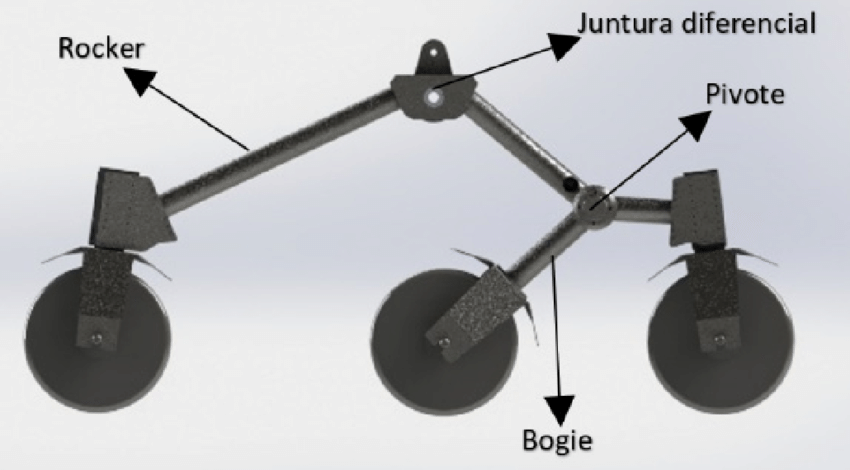
\includegraphics[width=.9\textwidth]{fig/rb-suspension.png}
    \end{figure}
    \vspace{5mm}
    \begin{figure}[ht]
      \centering
      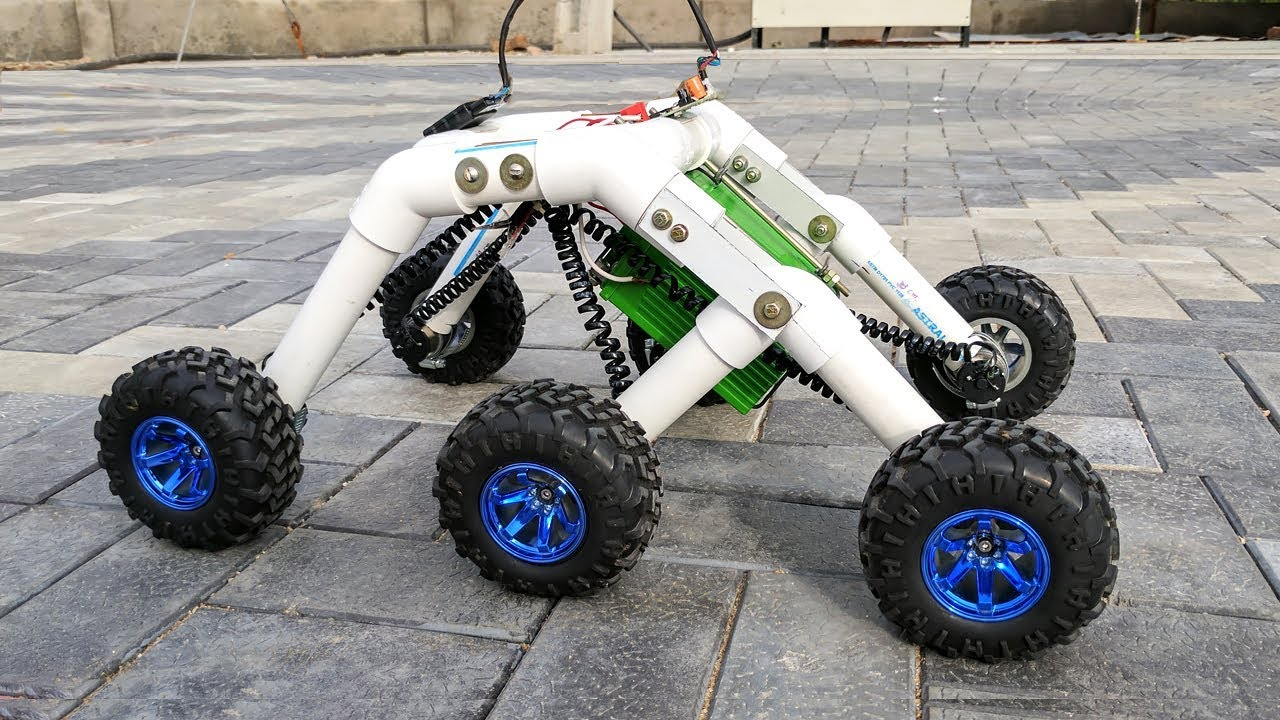
\includegraphics[width=.9\textwidth]{fig/rb.jpg}
    \end{figure}
  \end{columns}
\end{frame}

\begin{frame}{Uso do sistema de suspensão}
  % \vspace{12mm}
  \begin{figure}[ht]
    \begin{minipage}[b]{.32\textwidth}
      \centering
      Sojourner (1996)
      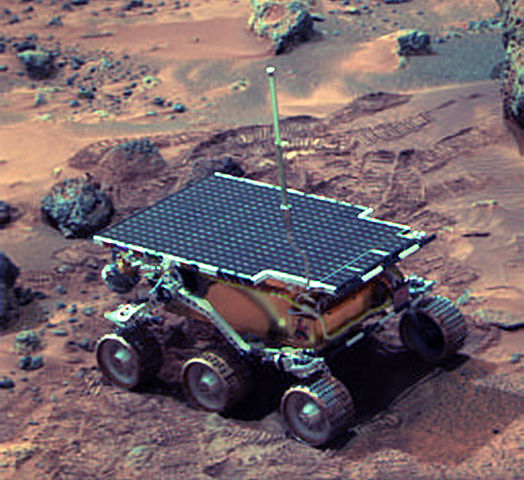
\includegraphics[width=.9\textwidth,height=2.8cm]{fig/sojourner.jpg}
    \end{minipage}%
    \begin{minipage}[b]{.32\textwidth}
      \centering
      Spirit (2003)
      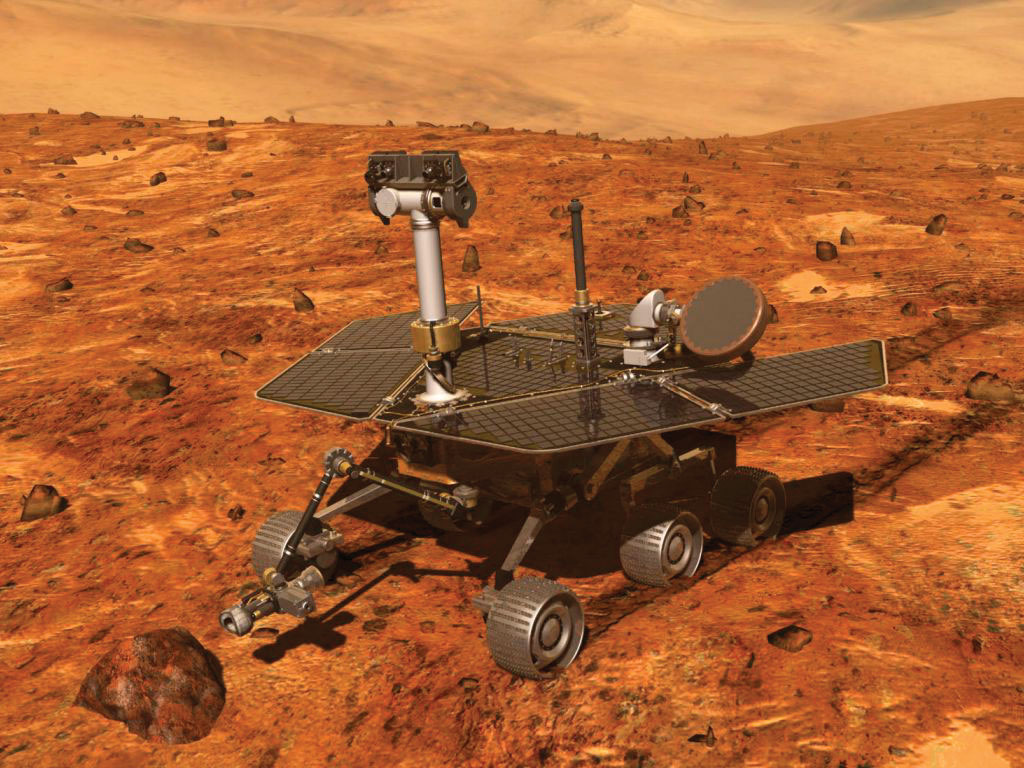
\includegraphics[width=.9\textwidth,height=2.8cm]{fig/spirit.jpg}
    \end{minipage}%
    \begin{minipage}[b]{.32\textwidth}
      \centering
      Opportunity (2003)
      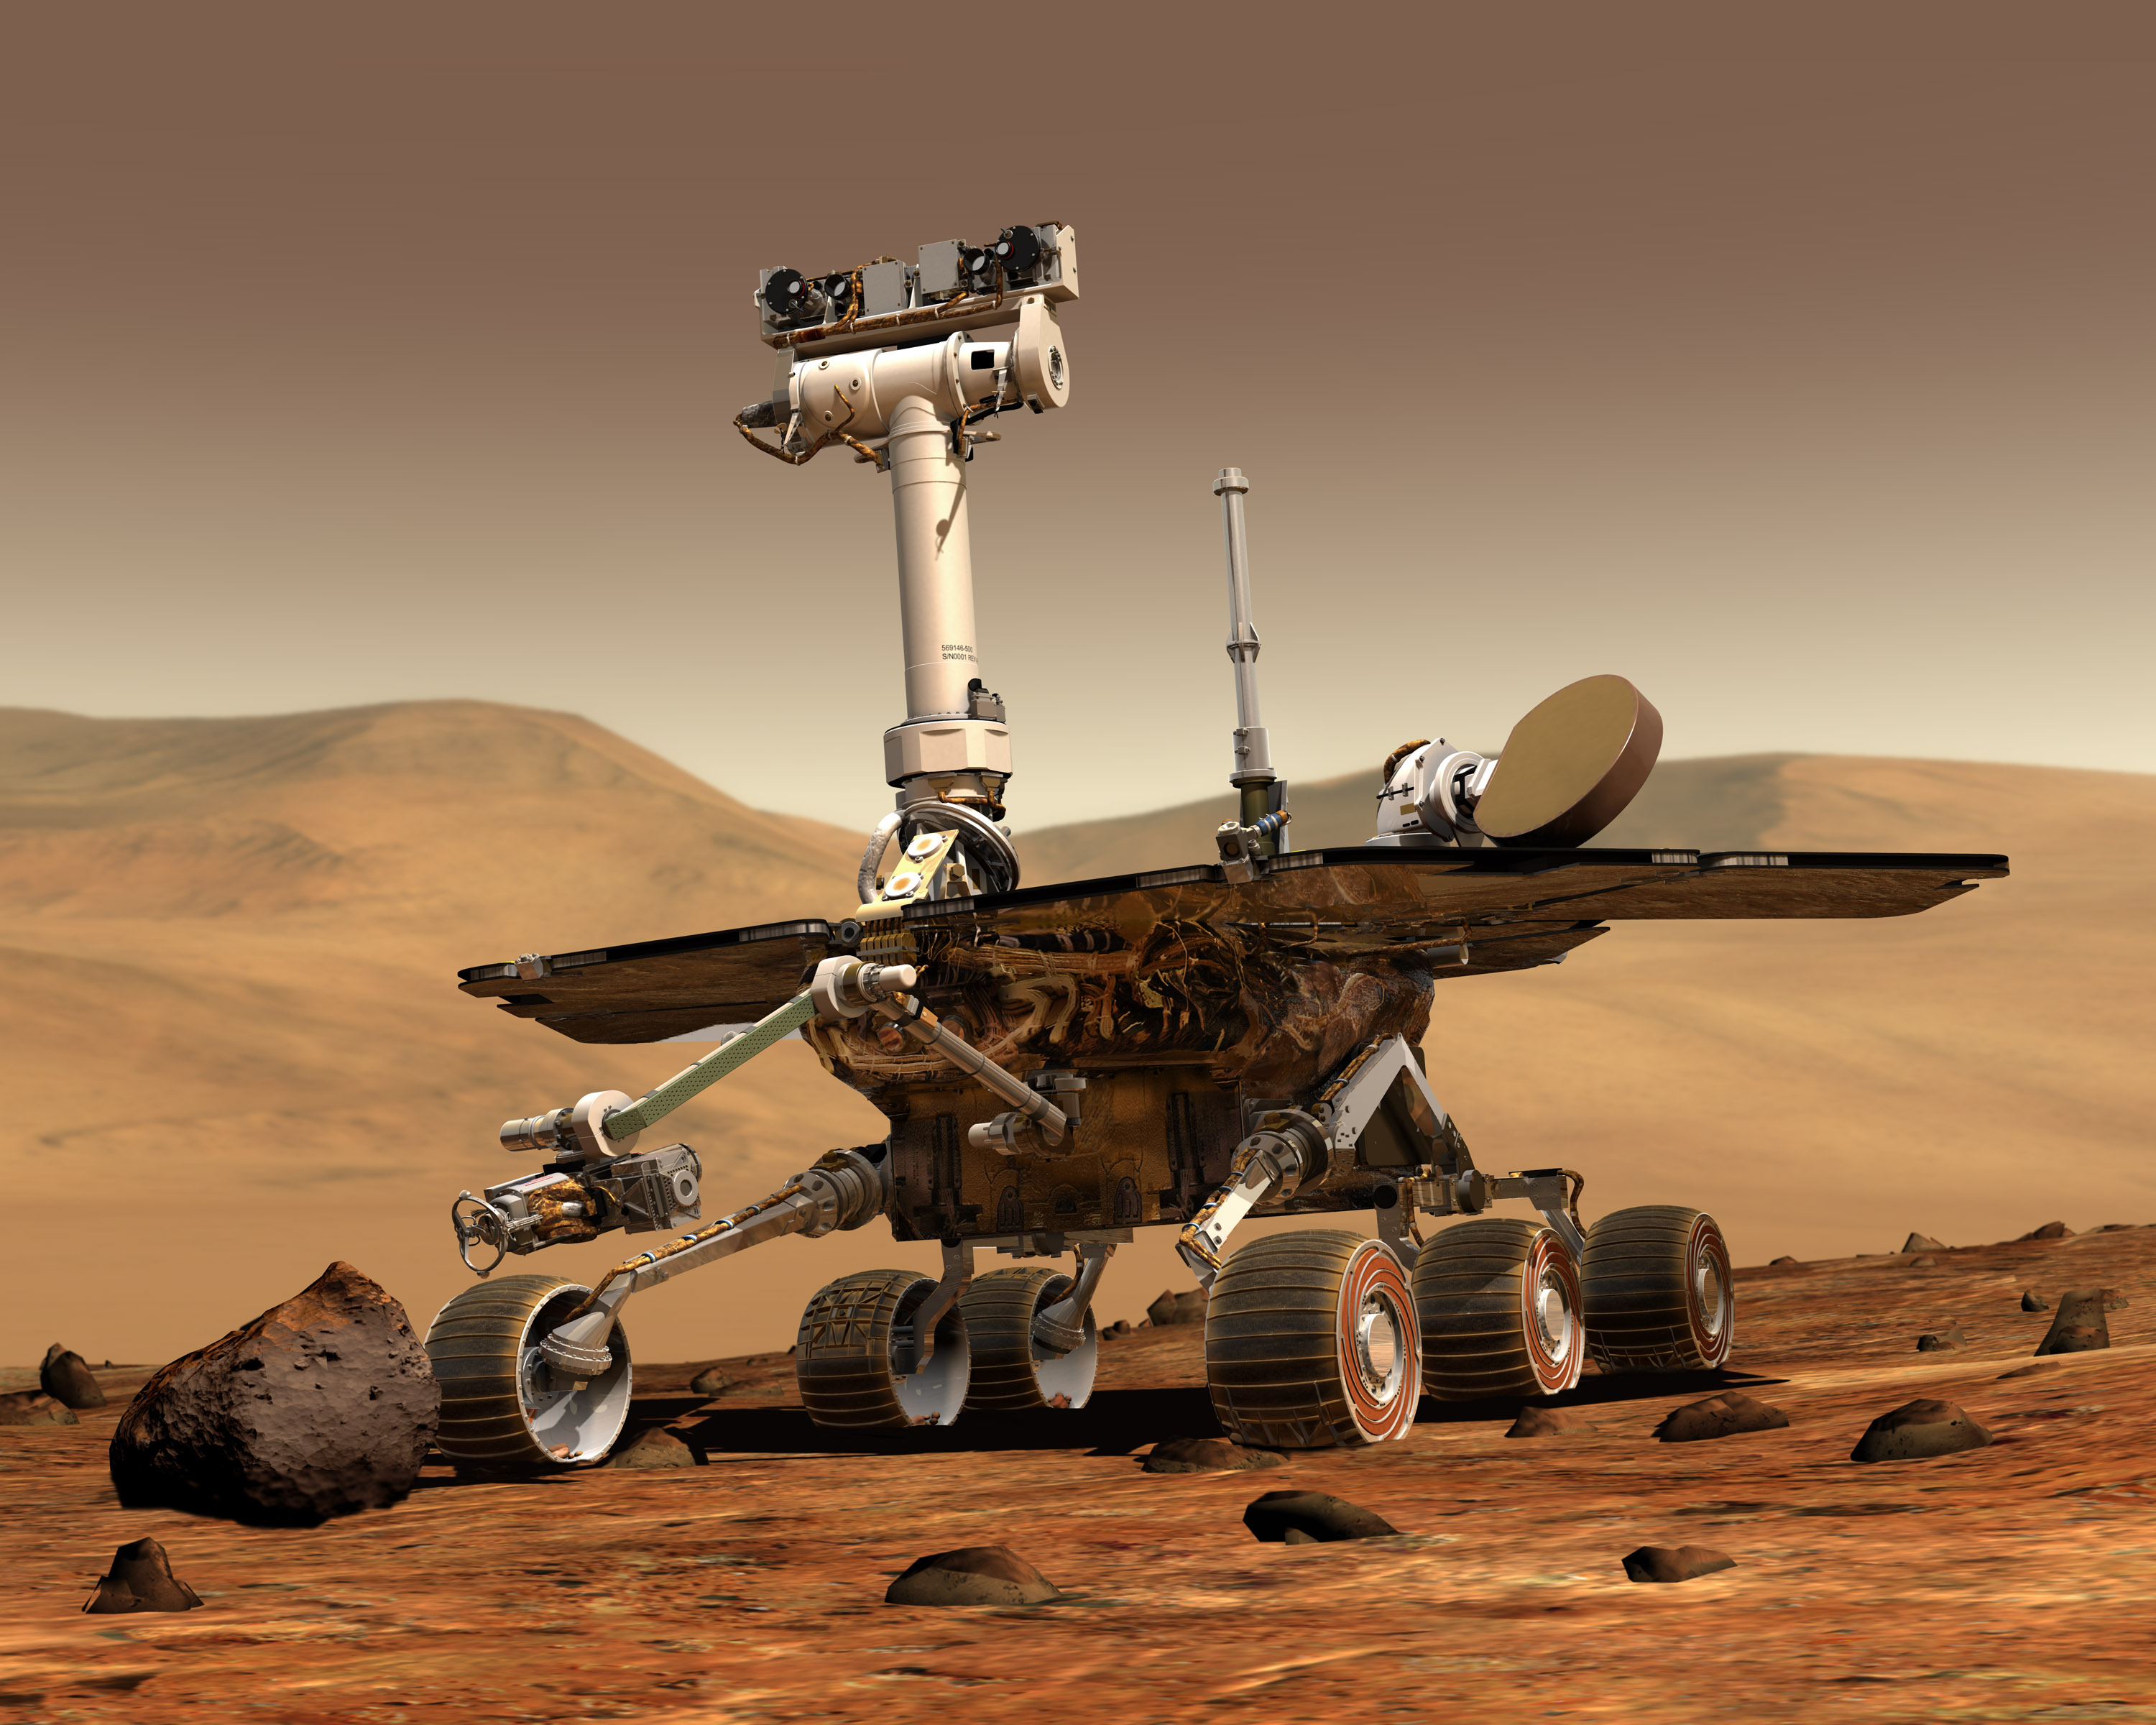
\includegraphics[width=.9\textwidth,height=2.8cm]{fig/opportunity.jpg}
    \end{minipage}
  \end{figure}
  \vspace{-4mm}
  \begin{figure}[ht]
    \begin{minipage}[b]{.32\textwidth}
      \centering
      Curiosity (2011)
      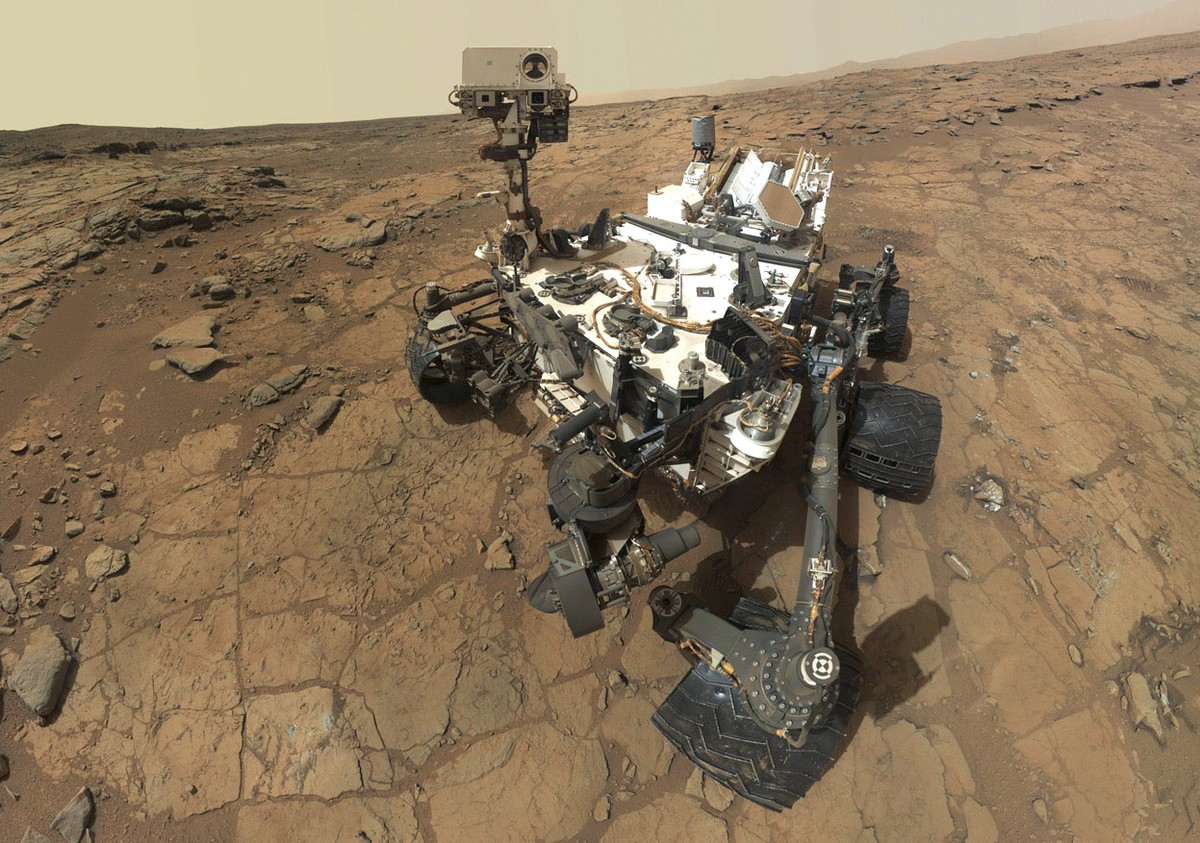
\includegraphics[width=.9\textwidth,height=2.8cm,trim={11cm 0 6.5cm 0},clip]{fig/curiosity.jpg}
    \end{minipage}%
    \hspace{5mm}
    \begin{minipage}[b]{.32\textwidth}
      \centering
      Perseverance (2020)
      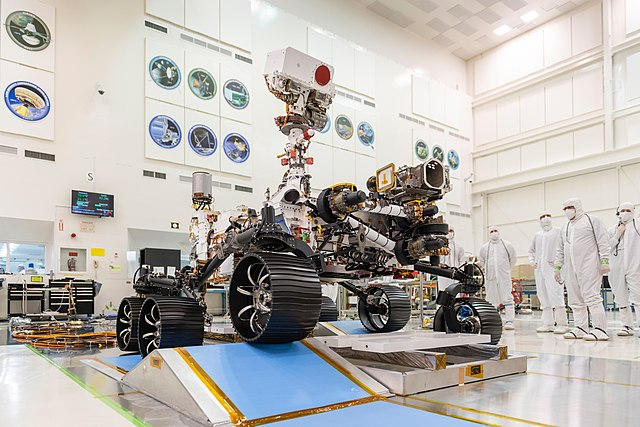
\includegraphics[width=.9\textwidth,height=2.8cm]{fig/perseverance.jpg}
    \end{minipage}%
  \end{figure}
\end{frame}

\section{Análise da Estrutura}

\begin{frame}{Diagrama da Estrutura}
  \begin{figure}[ht]
    \centering
    \resizebox{.8\textwidth}{!}{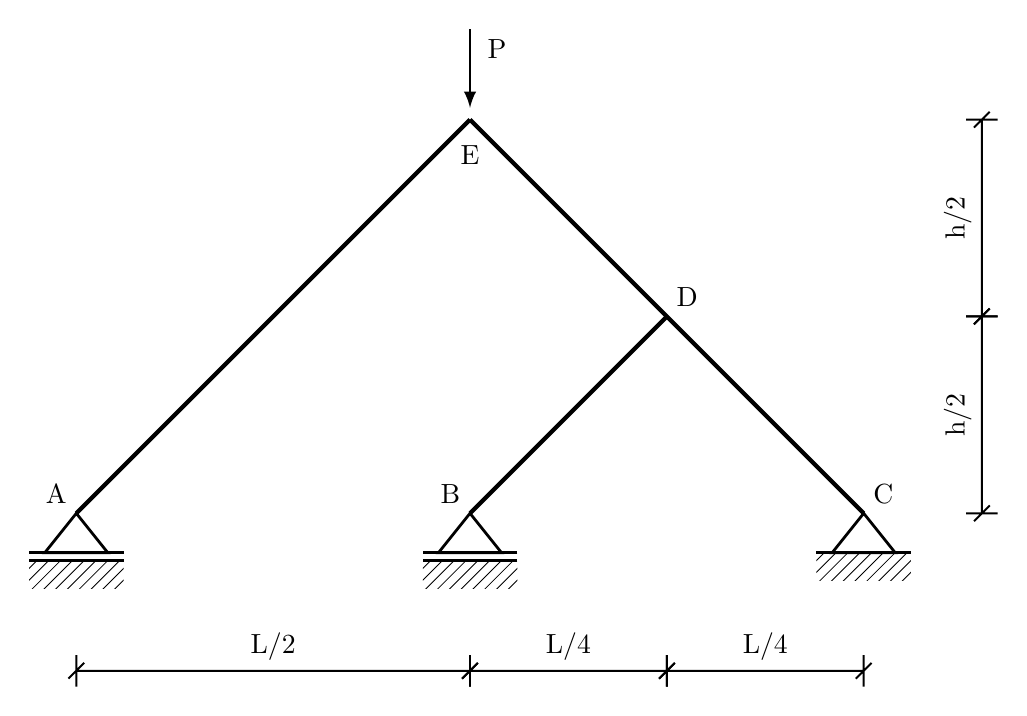
\begin{tikzpicture}
  \begin{scope}
    \point{a}{0}{0};
    \point{b}{5}{0};
    \point{c}{10}{0};
    \point{d}{7.5}{2.5};
    \point{e}{5}{5};

    \beam{2}{a}{e};
    \beam{2}{e}{c};
    \beam{2}{d}{b};

    \support{2}{a};
    \support{2}{b};
    \support{1}{c};

    \dimensioning{1}{a}{b}{-2}[L/2];
    \dimensioning{1}{b}{d}{-2}[L/4];
    \dimensioning{1}{d}{c}{-2}[L/4];
    \dimensioning{2}{d}{e}{11.5}[h/2];
    \dimensioning{2}{c}{d}{11.5}[h/2];

    \load{1}{e}[90];

    \dnotation{1}{e}{P}[yshift=9mm,right=1mm];
    \dnotation{1}{a}{A}[above left];
    \dnotation{1}{b}{B}[above left];
    \dnotation{1}{c}{C}[above right];
    \dnotation{1}{d}{D}[above right];
    \dnotation{1}{e}{E}[below=2mm];
  \end{scope}
\end{tikzpicture}}
  \end{figure}
\end{frame}

\begin{frame}{Simplificação}
  \begin{figure}[ht]
    \centering
    \resizebox{.8\textwidth}{!}{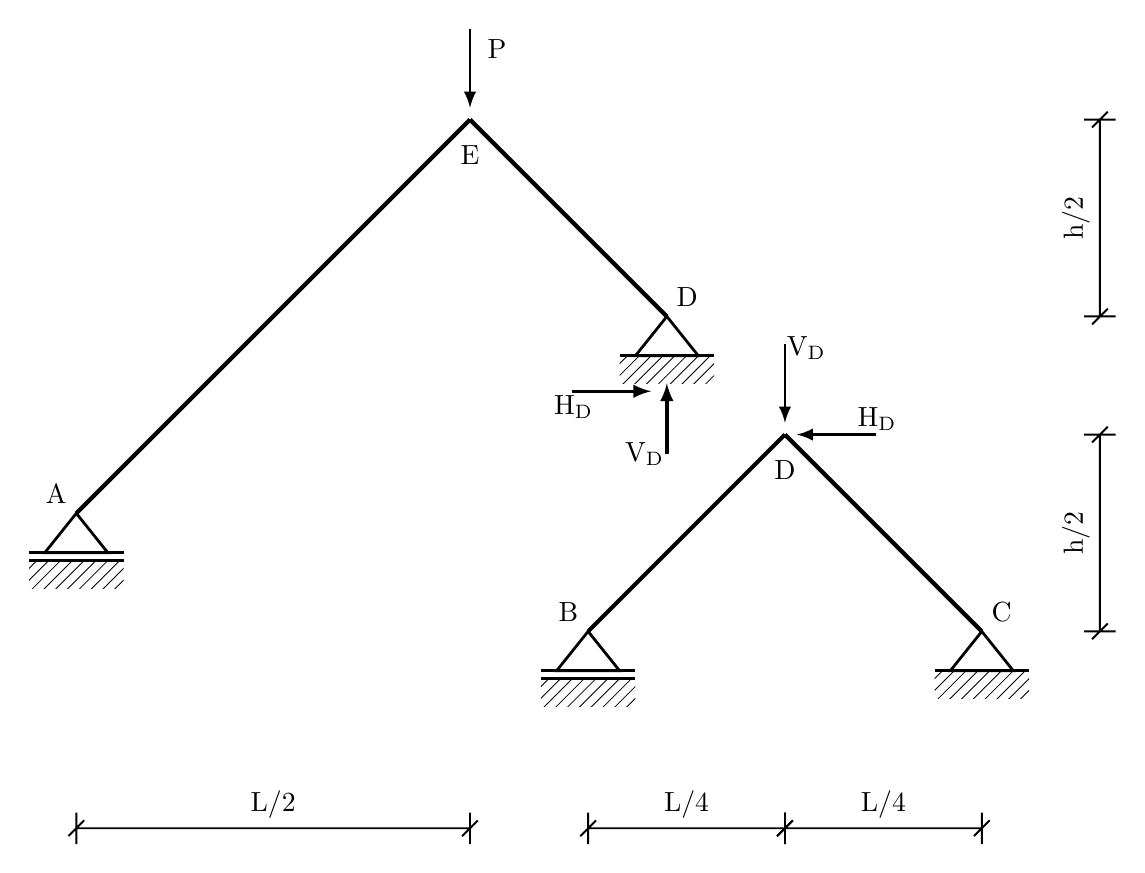
\begin{tikzpicture}
  \begin{scope}
    \point{a}{0}{0};
    \point{b}{6.5}{-1.5};
    \point{c}{11.5}{-1.5};
    \point{d1}{7.5}{2.5};
    \point{d2}{9}{1};
    \point{e}{5}{5};

    \beam{2}{a}{e};
    \beam{2}{d1}{e};
    \beam{2}{b}{d2};
    \beam{2}{c}{d2};

    \support{2}{a};
    \support{2}{b};
    \support{1}{c};
    \support{1}{d1};

    \dimensioning{1}{a}{e}{-4}[L/2];
    \dimensioning{1}{b}{d2}{-4}[L/4];
    \dimensioning{1}{d2}{c}{-4}[L/4];
    \dimensioning{2}{d1}{e}{13}[h/2];
    \dimensioning{2}{c}{d2}{13}[h/2];

    \load{1}{e}[90];

    \dnotation{1}{e}{P}[yshift=9mm,right=1mm];
    \dnotation{1}{a}{A}[above left];
    \dnotation{1}{b}{B}[above left];
    \dnotation{1}{c}{C}[above right];
    \dnotation{1}{d1}{D}[above right];
    \dnotation{1}{d2}{D}[below=2mm];
    \dnotation{1}{e}{E}[below=2mm];

    \draw[-{latex[scale=3.0]},very thick] (7.5,0.75) -- (7.5,1.65) node[yshift=-3mm,left=8mm] {H\textsubscript{D}};
    \draw[-{latex[scale=3.0]},very thick] (6.3,1.55) -- (7.3,1.55) node[yshift=-8mm,left=-3mm] {V\textsubscript{D}};
    \load{1}{d2}[90];
    \dnotation{1}{d2}{H\textsubscript{D}}[yshift=2mm,right=8mm];
    \load{1}{d2}[360];
    \dnotation{1}{d2}{V\textsubscript{D}}[yshift=11mm,right=-1mm];
  \end{scope}
\end{tikzpicture}}
  \end{figure}
\end{frame}

\begin{frame}{Análise da Primeira Estrutura}
  \begin{figure}[ht]
    \centering
    \resizebox{.75\textwidth}{!}{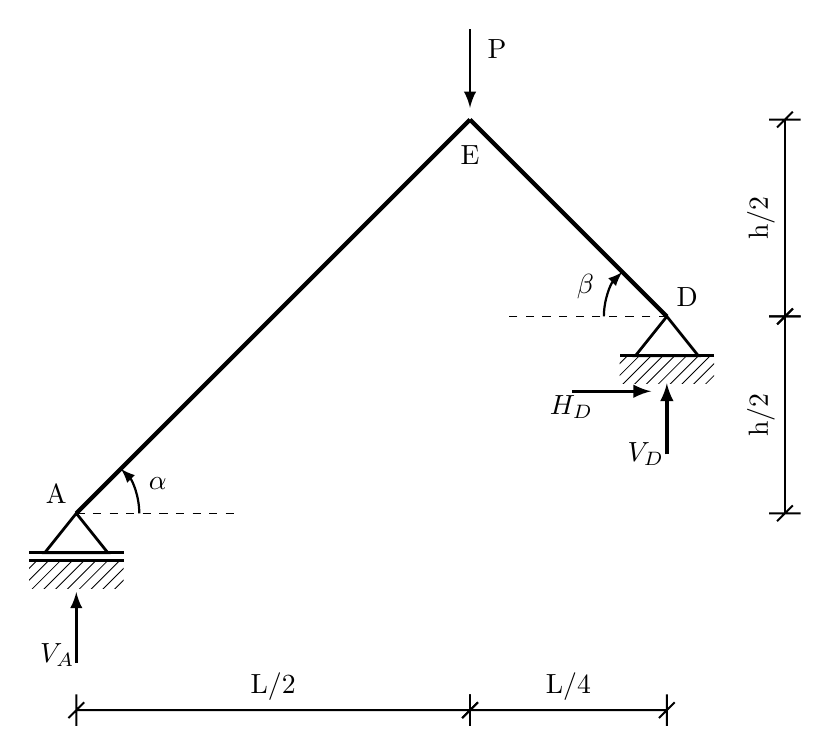
\begin{tikzpicture}
  \begin{scope}
    \point{a}{0}{0};
    \point{b}{6.5}{-1.5};
    \point{c}{11.5}{-1.5};
    \point{d1}{7.5}{2.5};
    \point{d2}{9}{1};
    \point{e}{5}{5};

    \beam{2}{a}{e};
    \beam{2}{d1}{e};

    \support{2}{a};
    \support{1}{d1};

    \dimensioning{1}{a}{e}{-2.5}[L/2];
    \dimensioning{1}{e}{d1}{-2.5}[L/4];
    \dimensioning{2}{a}{d1}{9}[h/2];
    \dimensioning{2}{d1}{e}{9}[h/2];

    \load{1}{e}[90];

    \dnotation{1}{e}{P}[yshift=9mm,right=1mm];
    \dnotation{1}{a}{A}[above left];
    \dnotation{1}{d1}{D}[above right];
    \dnotation{1}{e}{E}[below=2mm];

    \draw[-{latex[scale=3.0]},very thick] (7.5,0.75) -- (7.5,1.65) node[yshift=-3mm,left=8mm] {$H_D$};
    \draw[-{latex[scale=3.0]},very thick] (6.3,1.55) -- (7.3,1.55) node[yshift=-8mm,left=-3mm] {$V_D$};
    \load{1}{a}[270][.9][1];
    \dnotation{1}{a}{$V_A$}[left=-1mm,yshift=-18mm];

    \draw[-{latex[scale=3.0]},thick] (.8,0) arc (0:45:.8) node[] at (20:1.1) {$\alpha$};
    \draw[dashed] (0,0) -- (2,0);
    \draw[-{latex[scale=3.0]},thick] (6.7,2.5) arc (180:135:.8) node[shift=({7.5,2.5})] at (160:1.1) {$\beta$};
    \draw[dashed] (7.5,2.5) -- (5.5,2.5);
  \end{scope}
\end{tikzpicture}}
  \end{figure}
\end{frame}

\begin{frame}{Equações de Equilíbrio}
  \begin{columns}
    \column{.65\textwidth}
    \scriptsize
    \centering
    \begin{empheq}[left=\empheqlbrace]{align*}
      &\quad\sum F_H = 0 \;\Rightarrow\; H_D = 0\\
      &\quad\sum F_V = 0 \;\Rightarrow\; V_A + V_D - P = 0\\
      &\quad\sum M_A = 0 \;\Rightarrow\; \left(\frac{L}{2} + \frac{L}{4}\right)V_D - \frac{L}{2}P - \frac{h}{2}H_D = 0\\
      &\quad\sum M_D = 0 \;\Rightarrow\; \left(\frac{L}{2} + \frac{L}{4}\right)V_A + \frac{L}{4}P = 0
    \end{empheq}
    $\boxed{H_D = 0}$ \qquad $\boxed{V_A = \frac{P}{3}}$ \qquad $\boxed{V_D = \frac{2P}{3}}$
    \column{.35\textwidth}
    \begin{figure}[ht]
      \centering
      \resizebox{\textwidth}{!}{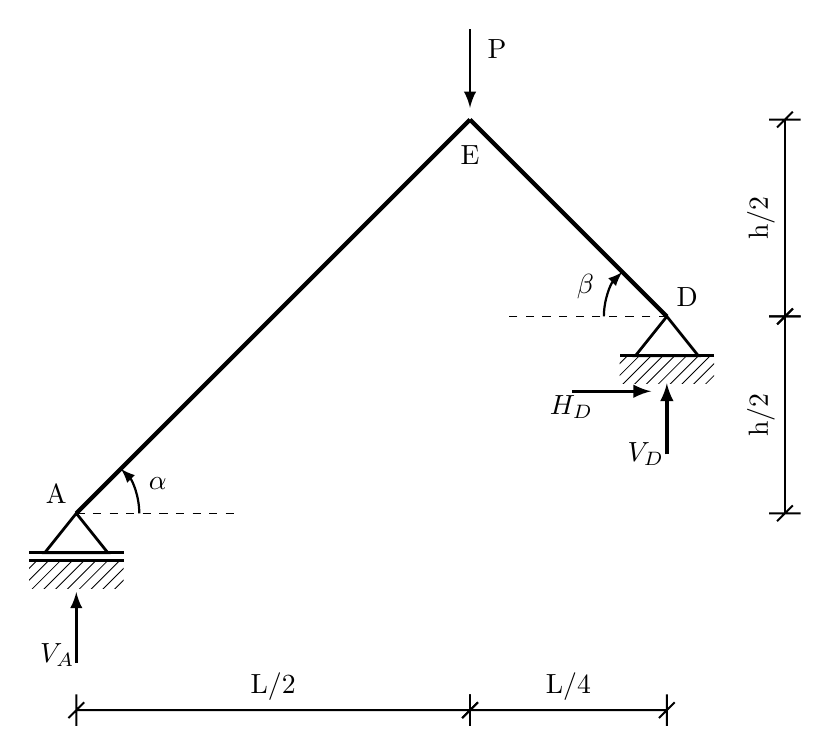
\begin{tikzpicture}
  \begin{scope}
    \point{a}{0}{0};
    \point{b}{6.5}{-1.5};
    \point{c}{11.5}{-1.5};
    \point{d1}{7.5}{2.5};
    \point{d2}{9}{1};
    \point{e}{5}{5};

    \beam{2}{a}{e};
    \beam{2}{d1}{e};

    \support{2}{a};
    \support{1}{d1};

    \dimensioning{1}{a}{e}{-2.5}[L/2];
    \dimensioning{1}{e}{d1}{-2.5}[L/4];
    \dimensioning{2}{a}{d1}{9}[h/2];
    \dimensioning{2}{d1}{e}{9}[h/2];

    \load{1}{e}[90];

    \dnotation{1}{e}{P}[yshift=9mm,right=1mm];
    \dnotation{1}{a}{A}[above left];
    \dnotation{1}{d1}{D}[above right];
    \dnotation{1}{e}{E}[below=2mm];

    \draw[-{latex[scale=3.0]},very thick] (7.5,0.75) -- (7.5,1.65) node[yshift=-3mm,left=8mm] {$H_D$};
    \draw[-{latex[scale=3.0]},very thick] (6.3,1.55) -- (7.3,1.55) node[yshift=-8mm,left=-3mm] {$V_D$};
    \load{1}{a}[270][.9][1];
    \dnotation{1}{a}{$V_A$}[left=-1mm,yshift=-18mm];

    \draw[-{latex[scale=3.0]},thick] (.8,0) arc (0:45:.8) node[] at (20:1.1) {$\alpha$};
    \draw[dashed] (0,0) -- (2,0);
    \draw[-{latex[scale=3.0]},thick] (6.7,2.5) arc (180:135:.8) node[shift=({7.5,2.5})] at (160:1.1) {$\beta$};
    \draw[dashed] (7.5,2.5) -- (5.5,2.5);
  \end{scope}
\end{tikzpicture}}
    \end{figure}
  \end{columns}
\end{frame}

\begin{frame}{Teorema do Corte: A-E}
  \begin{columns}
    \column{.35\textwidth}
    \begin{figure}[ht]
      \centering
      \resizebox{\textwidth}{!}{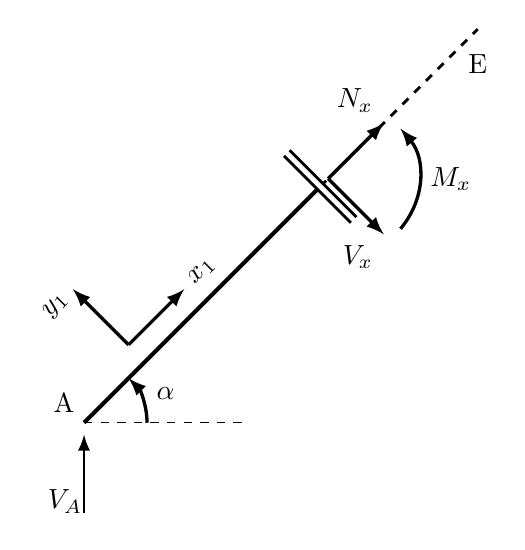
\begin{tikzpicture}
  \tikzstyle{arr}=[-{latex[scale=3.0]},very thick];

  \begin{scope}
    \point{i}{0}{0};
    \point{f}{5}{5};
    \point{x}{3}{3};

    \dnotation{1}{i}{A}[above left];
    \dnotation{1}{f}{E}[below=2mm];

    \load{1}{i}[270];
    \dnotation{1}{i}{$V_A$}[left=-1mm,yshift=-10mm];

    \draw[arr] (.8,0) arc (0:45:.8) node[] at (20:1.1) {$\alpha$};
    \draw[dashed] (0,0) -- (2,0);

    \beam{2}{i}{x};
    \beam{3}{x}{f};
    \hinge{3}{x}[45];
  \end{scope}

  \begin{scope}[rotate=45,shift=({1.1,.3})]
    \draw[arr] (0,0) -- (0,1) node[left,rotate=45] {$y_1$};
    \draw[arr] (0,0) -- (1,0) node[right,rotate=45] {$x_1$};
  \end{scope}

  \begin{scope}[shift=({3.1,3.1}),rotate=-45]
    \draw[arr] (0,0) -- (0,1) node[above left] {$N_x$};
    \draw[arr] (0,0) -- (1,0) node[below left] {$V_x$};
    \path[arr] (1.1,.2) edge [bend right=40] node[right] {$M_x$} (.2,1.1);
  \end{scope}

\end{tikzpicture}}
      \resizebox{.5\textwidth}{!}{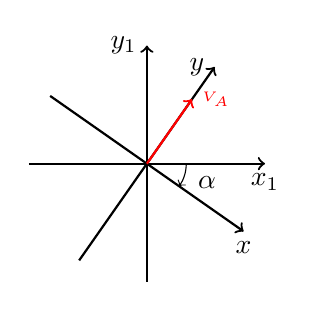
\begin{tikzpicture}
  \begin{scope}
    \draw[->,thick] (-1.5,0) -- (1.5,0) node[below] {$x_1$};
    \draw[->,thick] (0,-1.5) -- (0,1.5) node[left] {$y_1$};
    \draw[->,thick,rotate=-35] (-1.5,0) -- (1.5,0) node[below] {$x$};
    \draw[->,thick,rotate=-35] (0,-1.5) -- (0,1.5) node[left] {$y$};
    \draw[->] (.5,0) arc (0:-35:.5) node at (-17:.8) {$\alpha$};
    \draw[->,thick,red,rotate=-35] (0,0) -- (0,1) node[right] {\tiny $V_A$};
  \end{scope}
\end{tikzpicture}}
    \end{figure}
    \column{.65\textwidth}
    \scriptsize
    \centering
    \begin{empheq}[left=\empheqlbrace]{align*}
      &\sum F_H = 0 \;\Rightarrow\; V_A\sin\alpha + N_x = 0\\
      &\sum F_V = 0 \;\Rightarrow\; V_A\cos\alpha + V_x = 0\\
      &\sum M_x = 0 \;\Rightarrow\; -V_A\cos\alpha x + M_x = 0
    \end{empheq}
    $\boxed{N_x = -\frac{P}{3}\sin\alpha}$ \qquad $\boxed{V_x = \frac{P}{3}\cos\alpha}$
    $\boxed{M_x = \frac{P}{3}\cos\alpha x}$
  \end{columns}
\end{frame}

\begin{frame}{Teorema do Corte: D-E}
  \begin{columns}
    \column{.35\textwidth}
    \begin{figure}[ht]
      \centering
      \resizebox{\textwidth}{!}{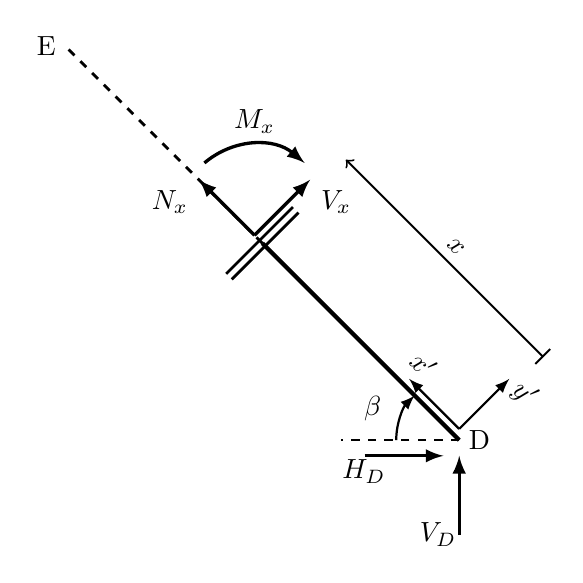
\begin{tikzpicture}
  \tikzstyle{arr}=[-{latex[scale=3.0]},very thick];
  \tikzstyle{arr2}=[-{latex[scale=3.0]},thick];

  \begin{scope}
    \point{i}{10}{0};
    \point{f}{5}{5};
    \point{x}{7.5}{2.5};

    \dnotation{1}{i}{D}[right];
    \dnotation{1}{f}{E}[left];

    \draw[arr] ($(i) - (0,1.2)$) -- ($(i) - (0,.2)$) node[yshift=-2mm,left=8mm] {$H_D$};
    \draw[arr] ($(i) - (1.2,.2)$) -- ($(i) - (.2,.2)$) node[yshift=-10mm,left=-3mm] {$V_D$};

    \draw[arr2] ($(i) - (.8,0)$) arc (180:135:.8) node[shift={($(i) + (-1.1,.4)$)}] at (160:1.1) {$\beta$};
    \draw[dashed] (i) -- ($(i) - (1.5,0)$);

    \hinge{3}{x}[135];
    \beam{2}{i}{x};
    \beam{3}{x}{f};

    \dimensioning{3}{i}{x}{-1.5}[$x$];
  \end{scope}

  \begin{scope}[rotate=-45,shift={($(i)+(-.1,.1)$)}] %{1.1,.3}
    \draw[arr2] (0,0) -- (0,.9) node[right,rotate=-45] {$y'$};
    \draw[arr2] (0,0) -- (-.9,0) node[anchor=south,rotate=-45] {$x'$};
  \end{scope}

  \begin{scope}[shift={($(x) + (-.1,.1)$)},rotate=-45]
    \draw[arr] (0,0) -- (0,1) node[below right] {$V_x$};
    \draw[arr] (0,0) -- (-1,0) node[below left] {$N_x$};
    \path[arr] (-1.1,.2) edge [bend left=40] node[anchor=south] {$M_x$} (-0.2,1.1);
  \end{scope}
\end{tikzpicture}}
    \end{figure}
    \column{.65\textwidth}
    \scriptsize
    \centering
    \begin{empheq}[left=\empheqlbrace]{align*}
      &\quad\sum F_H = 0 \;\Rightarrow\; V_D\sin\beta - H_D\cos\beta + N_x = 0\\
      &\quad\sum F_V = 0 \;\Rightarrow\; V_D\cos\beta + H_D\sin\beta - V_x = 0\\
      &\quad\sum M_x = 0 \;\Rightarrow\; (V_D\cos\beta + H_D\sin\beta)x - M_x = 0
    \end{empheq}
    $\boxed{N_x = -\frac{2P}{3}\sin\beta}$ \qquad $\boxed{V_x = \frac{2P}{3}\cos\beta}$
    $\boxed{M_x = \frac{2P}{3}\cos\beta x}$
  \end{columns}
\end{frame}

\begin{frame}{Análise da Segunda Estrutura}
  \begin{figure}[ht]
    \centering
    \resizebox{.75\textwidth}{!}{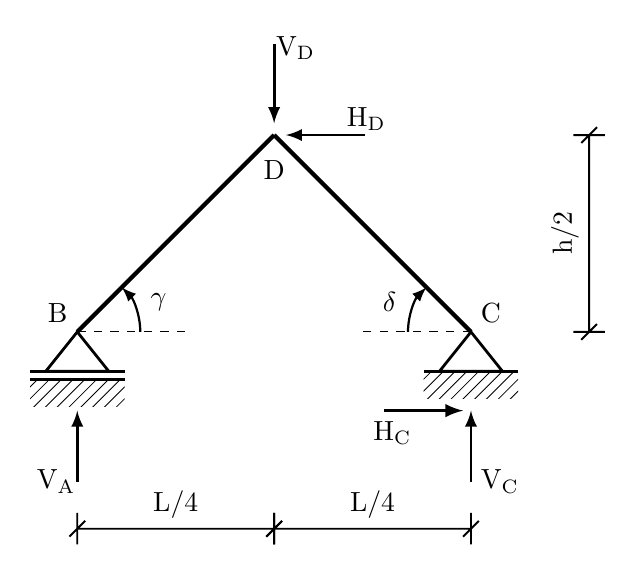
\begin{tikzpicture}
  \begin{scope}
    \point{a}{0}{0};
    \point{b}{6.5}{-1.5};
    \point{c}{11.5}{-1.5};
    \point{d1}{7.5}{2.5};
    \point{d2}{9}{1};
    \point{e}{5}{5};

    \beam{2}{b}{d2};
    \beam{2}{c}{d2};

    \support{2}{b};
    \support{1}{c};

    \dimensioning{1}{b}{d2}{-4}[L/4];
    \dimensioning{1}{d2}{c}{-4}[L/4];
    \dimensioning{2}{c}{d2}{13}[h/2];

    \dnotation{1}{b}{B}[above left];
    \dnotation{1}{c}{C}[above right];
    \dnotation{1}{d2}{D}[below=2mm];

    \load{1}{d2}[90];
    \dnotation{1}{d2}{H\textsubscript{D}}[yshift=2mm,right=8mm];
    \load{1}{d2}[360];
    \dnotation{1}{d2}{V\textsubscript{D}}[yshift=11mm,right=-1mm];
    \load{1}{b}[270][.9][1];
    \dnotation{1}{b}{V\textsubscript{A}}[left=-1mm,yshift=-19mm];
    \load{1}{c}[270][.9][1];
    \dnotation{1}{c}{V\textsubscript{C}}[right,yshift=-19mm];
    \draw[-{latex[scale=3.0]},very thick] (10.4,-2.5) -- (11.4,-2.5) node[below,xshift=-9mm] {H\textsubscript{C}};

    \draw[-{latex[scale=3.0]},thick] (7.3,-1.5) arc (0:45:.8) node[shift=({6.5,-1.5})] at (20:1.1) {$\gamma$};
    \draw[dashed] (6.5,-1.5) -- (7.9,-1.5);
    \draw[-{latex[scale=3.0]},thick] (10.7,-1.5) arc (180:135:.8) node[shift=({11.5,-1.5})] at (160:1.1) {$\delta$};
    \draw[dashed] (11.5,-1.5) -- (10.1,-1.5);
  \end{scope}
\end{tikzpicture}}
  \end{figure}
\end{frame}

\begin{frame}{Equações de Equilíbrio}
  \begin{columns}
    \column{.65\textwidth}
    \scriptsize
    \centering
    \begin{empheq}[left=\empheqlbrace]{align*}
      &\sum F_H = 0 \;\Rightarrow\; -H_D + H_C = 0\\
      &\sum F_V = 0 \;\Rightarrow\; V_B + V_C - V_D = 0\\
      &\sum M_B = 0 \;\Rightarrow\; \frac{L}{2}V_C - \frac{L}{4}V_D = 0\\
      &\sum M_C = 0 \;\Rightarrow\; -\frac{L}{2}V_B + \frac{L}{4}V_D = 0
    \end{empheq}
    $\boxed{H_C = 0}$ \qquad $\boxed{V_B = \frac{P}{3}}$ \qquad $\boxed{V_C = \frac{P}{3}}$
    \column{.35\textwidth}
    \begin{figure}[ht]
      \centering
      \resizebox{\textwidth}{!}{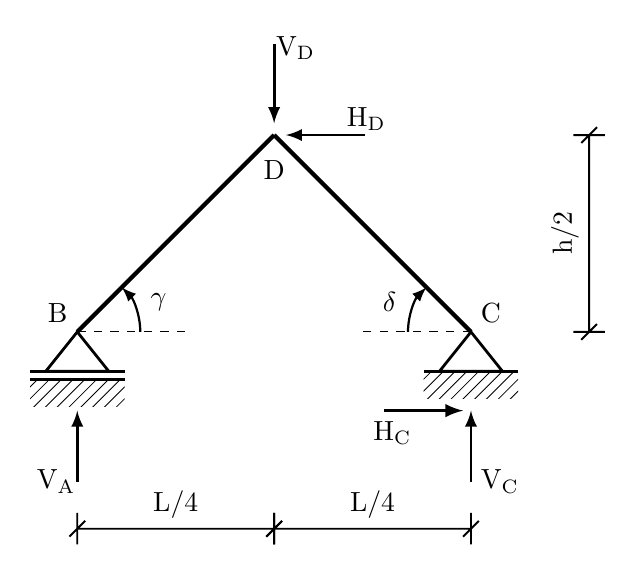
\begin{tikzpicture}
  \begin{scope}
    \point{a}{0}{0};
    \point{b}{6.5}{-1.5};
    \point{c}{11.5}{-1.5};
    \point{d1}{7.5}{2.5};
    \point{d2}{9}{1};
    \point{e}{5}{5};

    \beam{2}{b}{d2};
    \beam{2}{c}{d2};

    \support{2}{b};
    \support{1}{c};

    \dimensioning{1}{b}{d2}{-4}[L/4];
    \dimensioning{1}{d2}{c}{-4}[L/4];
    \dimensioning{2}{c}{d2}{13}[h/2];

    \dnotation{1}{b}{B}[above left];
    \dnotation{1}{c}{C}[above right];
    \dnotation{1}{d2}{D}[below=2mm];

    \load{1}{d2}[90];
    \dnotation{1}{d2}{H\textsubscript{D}}[yshift=2mm,right=8mm];
    \load{1}{d2}[360];
    \dnotation{1}{d2}{V\textsubscript{D}}[yshift=11mm,right=-1mm];
    \load{1}{b}[270][.9][1];
    \dnotation{1}{b}{V\textsubscript{A}}[left=-1mm,yshift=-19mm];
    \load{1}{c}[270][.9][1];
    \dnotation{1}{c}{V\textsubscript{C}}[right,yshift=-19mm];
    \draw[-{latex[scale=3.0]},very thick] (10.4,-2.5) -- (11.4,-2.5) node[below,xshift=-9mm] {H\textsubscript{C}};

    \draw[-{latex[scale=3.0]},thick] (7.3,-1.5) arc (0:45:.8) node[shift=({6.5,-1.5})] at (20:1.1) {$\gamma$};
    \draw[dashed] (6.5,-1.5) -- (7.9,-1.5);
    \draw[-{latex[scale=3.0]},thick] (10.7,-1.5) arc (180:135:.8) node[shift=({11.5,-1.5})] at (160:1.1) {$\delta$};
    \draw[dashed] (11.5,-1.5) -- (10.1,-1.5);
  \end{scope}
\end{tikzpicture}}
    \end{figure}
  \end{columns}
\end{frame}

\begin{frame}{Teorema do Corte: C-D}
  \begin{columns}
    \column{.35\textwidth}
    \begin{figure}[ht]
      \centering
      \resizebox{\textwidth}{!}{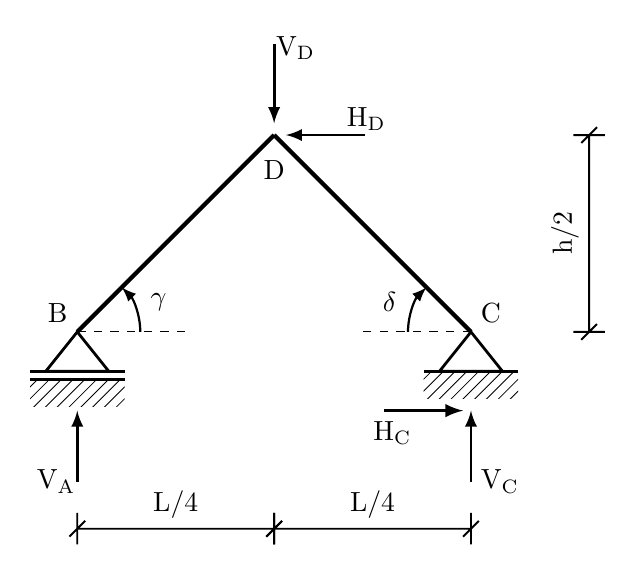
\begin{tikzpicture}
  \begin{scope}
    \point{a}{0}{0};
    \point{b}{6.5}{-1.5};
    \point{c}{11.5}{-1.5};
    \point{d1}{7.5}{2.5};
    \point{d2}{9}{1};
    \point{e}{5}{5};

    \beam{2}{b}{d2};
    \beam{2}{c}{d2};

    \support{2}{b};
    \support{1}{c};

    \dimensioning{1}{b}{d2}{-4}[L/4];
    \dimensioning{1}{d2}{c}{-4}[L/4];
    \dimensioning{2}{c}{d2}{13}[h/2];

    \dnotation{1}{b}{B}[above left];
    \dnotation{1}{c}{C}[above right];
    \dnotation{1}{d2}{D}[below=2mm];

    \load{1}{d2}[90];
    \dnotation{1}{d2}{H\textsubscript{D}}[yshift=2mm,right=8mm];
    \load{1}{d2}[360];
    \dnotation{1}{d2}{V\textsubscript{D}}[yshift=11mm,right=-1mm];
    \load{1}{b}[270][.9][1];
    \dnotation{1}{b}{V\textsubscript{A}}[left=-1mm,yshift=-19mm];
    \load{1}{c}[270][.9][1];
    \dnotation{1}{c}{V\textsubscript{C}}[right,yshift=-19mm];
    \draw[-{latex[scale=3.0]},very thick] (10.4,-2.5) -- (11.4,-2.5) node[below,xshift=-9mm] {H\textsubscript{C}};

    \draw[-{latex[scale=3.0]},thick] (7.3,-1.5) arc (0:45:.8) node[shift=({6.5,-1.5})] at (20:1.1) {$\gamma$};
    \draw[dashed] (6.5,-1.5) -- (7.9,-1.5);
    \draw[-{latex[scale=3.0]},thick] (10.7,-1.5) arc (180:135:.8) node[shift=({11.5,-1.5})] at (160:1.1) {$\delta$};
    \draw[dashed] (11.5,-1.5) -- (10.1,-1.5);
  \end{scope}
\end{tikzpicture}}
    \end{figure}
    \column{.65\textwidth}
    \scriptsize
    \centering
    \begin{empheq}[left=\empheqlbrace]{align*}
      &\quad\sum F_H = 0 \;\Rightarrow\; V_C\sin\gamma - H_C\cos\gamma + N_x = 0\\
      &\quad\sum F_V = 0 \;\Rightarrow\; H_C\sin\gamma + V_C\cos\gamma - V_x = 0\\
      &\quad\sum M_x = 0 \;\Rightarrow\; (H_C\sin\gamma + V_C\cos\gamma)x - M_x = 0
    \end{empheq}
    $\boxed{N_x = -\frac{P}{3}\sin\gamma}$ \qquad $\boxed{V_x = \frac{P}{3}\sin\gamma}$
    $\boxed{M_x = \frac{P}{3}\cos\gamma x}$
  \end{columns}
\end{frame}

\begin{frame}{Teorema do Corte: B-D}
  \begin{columns}
    \column{.35\textwidth}
    \begin{figure}[ht]
      \centering
      \resizebox{\textwidth}{!}{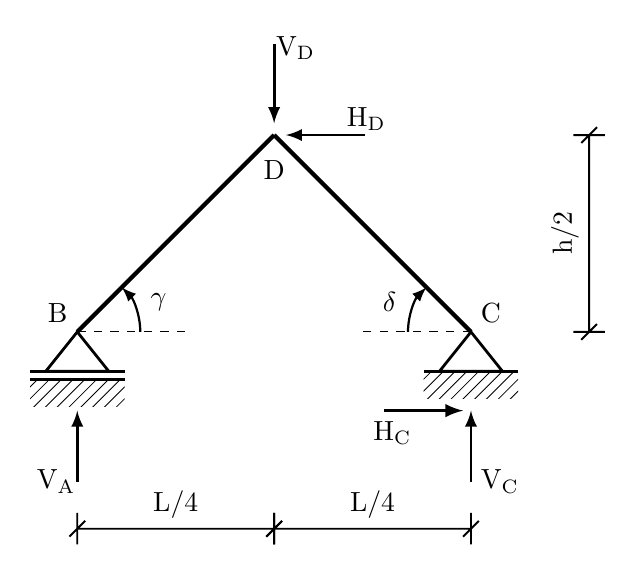
\begin{tikzpicture}
  \begin{scope}
    \point{a}{0}{0};
    \point{b}{6.5}{-1.5};
    \point{c}{11.5}{-1.5};
    \point{d1}{7.5}{2.5};
    \point{d2}{9}{1};
    \point{e}{5}{5};

    \beam{2}{b}{d2};
    \beam{2}{c}{d2};

    \support{2}{b};
    \support{1}{c};

    \dimensioning{1}{b}{d2}{-4}[L/4];
    \dimensioning{1}{d2}{c}{-4}[L/4];
    \dimensioning{2}{c}{d2}{13}[h/2];

    \dnotation{1}{b}{B}[above left];
    \dnotation{1}{c}{C}[above right];
    \dnotation{1}{d2}{D}[below=2mm];

    \load{1}{d2}[90];
    \dnotation{1}{d2}{H\textsubscript{D}}[yshift=2mm,right=8mm];
    \load{1}{d2}[360];
    \dnotation{1}{d2}{V\textsubscript{D}}[yshift=11mm,right=-1mm];
    \load{1}{b}[270][.9][1];
    \dnotation{1}{b}{V\textsubscript{A}}[left=-1mm,yshift=-19mm];
    \load{1}{c}[270][.9][1];
    \dnotation{1}{c}{V\textsubscript{C}}[right,yshift=-19mm];
    \draw[-{latex[scale=3.0]},very thick] (10.4,-2.5) -- (11.4,-2.5) node[below,xshift=-9mm] {H\textsubscript{C}};

    \draw[-{latex[scale=3.0]},thick] (7.3,-1.5) arc (0:45:.8) node[shift=({6.5,-1.5})] at (20:1.1) {$\gamma$};
    \draw[dashed] (6.5,-1.5) -- (7.9,-1.5);
    \draw[-{latex[scale=3.0]},thick] (10.7,-1.5) arc (180:135:.8) node[shift=({11.5,-1.5})] at (160:1.1) {$\delta$};
    \draw[dashed] (11.5,-1.5) -- (10.1,-1.5);
  \end{scope}
\end{tikzpicture}}
    \end{figure}
    \column{.65\textwidth}
    \scriptsize
    \centering
    \begin{empheq}[left=\empheqlbrace]{align*}
      &\quad\sum F_H = 0 \;\Rightarrow\; V_B\sin\beta + N_x\\
      &\quad\sum F_V = 0 \;\Rightarrow\; V_B\cos\beta - V_x\\
      &\quad\sum M_x = 0 \;\Rightarrow\; -V_B\cos\beta x + M_x = 0
    \end{empheq}
    $\boxed{N_x = -\frac{P}{3}\sin\beta}$ \qquad $\boxed{V_x = \frac{P}{3}\cos\beta}$
    $\boxed{M_x = \frac{P}{3}\cos\beta x}$
  \end{columns}
\end{frame}

\begin{frame}{Diagrama da Força Normal}
  \begin{figure}[ht]
    \centering
    \resizebox{.75\textwidth}{!}{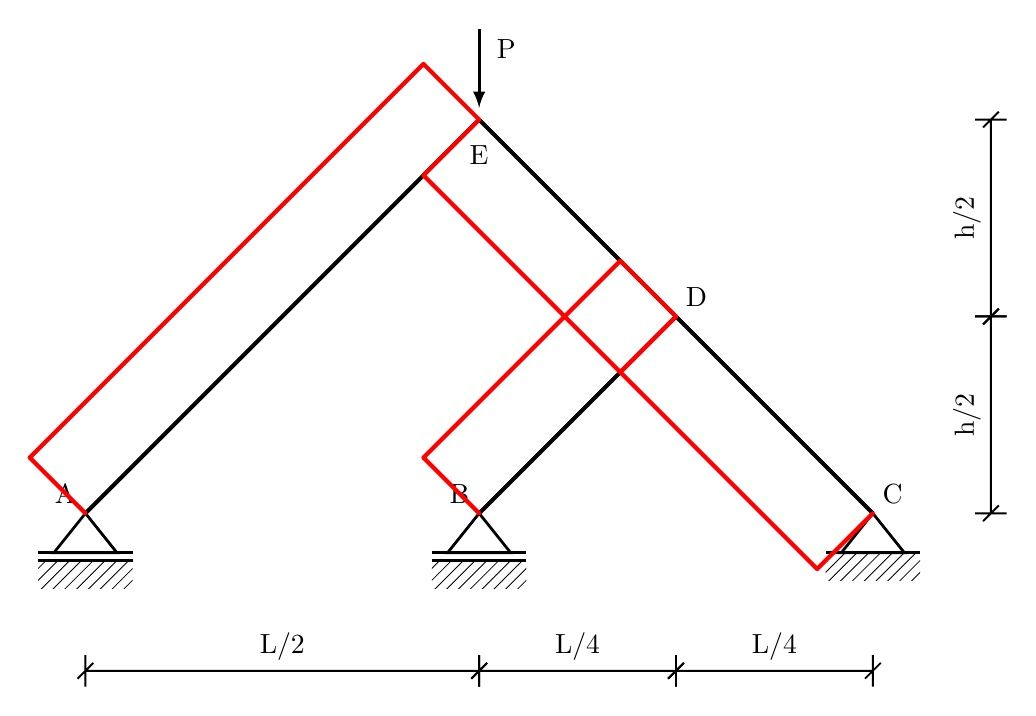
\begin{tikzpicture}
  \begin{scope}
    \point{a}{0}{0};
    \point{b}{5}{0};
    \point{c}{10}{0};
    \point{d}{7.5}{2.5};
    \point{e}{5}{5};

    \beam{2}{a}{e};
    \beam{2}{e}{c};
    \beam{2}{d}{b};

    \support{2}{a};
    \support{2}{b};
    \support{1}{c};

    \dimensioning{1}{a}{b}{-2}[L/2];
    \dimensioning{1}{b}{d}{-2}[L/4];
    \dimensioning{1}{d}{c}{-2}[L/4];
    \dimensioning{2}{d}{e}{11.5}[h/2];
    \dimensioning{2}{c}{d}{11.5}[h/2];

    \load{1}{e}[90];

    \dnotation{1}{e}{P}[yshift=9mm,right=1mm];
    \dnotation{1}{a}{A}[above left];
    \dnotation{1}{b}{B}[above left];
    \dnotation{1}{c}{C}[above right];
    \dnotation{1}{d}{D}[above right];
    \dnotation{1}{e}{E}[below=2mm];

    \internalforces{a}{e}{-1}{-1};
    \internalforces{d}{e}{-1}{-1};
    \internalforces{b}{d}{-1}{-1};
    \internalforces{c}{d}{-1}{-1};
  \end{scope}
\end{tikzpicture}}
  \end{figure}
\end{frame}

\end{document}